\documentclass{scrartcl}
\usepackage{amsmath}
\usepackage{amssymb}
\usepackage[geometry]{ifsym}
\usepackage{tikz}
\usetikzlibrary{positioning,calc}

\newcommand{\selection}{\sigma}
\newcommand{\projection}{\pi}
\newcommand{\rename}{\rho}
\newcommand{\join}{\mathbin{\text{\begin{tiny}\textifsym{|><|}\end{tiny}}}}
\newcommand{\fullouterjoin}{\mathbin{\text{\begin{tiny}\textifsym{d|><|d}\end{tiny}}}}
\newcommand{\leftouterjoin}{\mathbin{\text{\begin{tiny}\textifsym{d|><|}\end{tiny}}}}
\newcommand{\rightouterjoin}{\mathbin{\text{\begin{tiny}\textifsym{|><|d}\end{tiny}}}}
\newcommand{\semijoin}{\mathbin{\text{\begin{tiny}\textifsym{|><}\end{tiny}}}}
\newcommand{\groupby}{\Gamma}

\newcommand{\hyperedge}[4][180]{
     \draw (#2.#1) ++(#1:.5)  edge (#2) edge (#3) edge (#4);
}

\newcommand{\mtt}[1]{\text{\texttt{#1}}}

\setlength{\parindent}{0pt}

\begin{document}

\section*{Exercise 1}

Given the following query graph and a start solution calculated with GOO (see
also Exercise~1 of Homework~4):

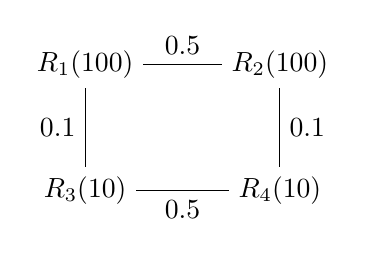
\begin{tikzpicture}
    \node (R1) {$R_1 (100)$};
    \node (R2) [right=of R1] {$R_2 (100)$};
    \node (R3) [below=of R1] {$R_3 (10)$};
    \node (R4) [below=of R2] {$R_4 (10)$};
    \draw
        (R1) to node [above] {$0.5$} (R2)
        (R1) to node [left] {$0.1$} (R3)
        (R2) to node [right] {$0.1$} (R4)
        (R3) to node [below] {$0.5$} (R4);
\end{tikzpicture}

GOO solution: $((R_3 \join R_4) \join R_2) \join R_1$, Cost: 3050

We will never get to the optimal solution $(R_1 \join R_3) \join (R_2 \join
R_4)$, which has cost 2700, when using the following rules seen in the lecture:
Commutativity, Right Associativity, Left Associativity, Left Join Exchange, and
Right Join Exchange.

The following table shows the steps needed to get to the optimal solution and
their cost:

\begin{table}[h]
    \centering
    \begin{tabular}{l|l|l}
        Rule & Result & Cost \\ \hline
        Commutativity & $((R_4 \join R_3) \join R_2) \join R_1$ & 3050 \\
        Left Join Exchange & $((R_4 \join R_2) \join R_3) \join R_1$ & 7600 \\
        Right Associativity & $(R_4 \join R_2) \join (R_3 \join R_1)$ & 2700
    \end{tabular}
\end{table}

Because the intermediate result after the Left Join Exchange is more expensive
than the result before, this path will not be taken when doing Iterative
Improvement, so the optimal solution will never be found.


\end{document}
